\documentclass[tikz,border=10pt]{standalone}
\usepackage{fontspec}
\setmainfont{IBM Plex Serif}
\usepackage{unicode-math}
\setmathfont{STIX Two Math}
\usepackage{pgfplots}
\pgfplotsset{compat=newest}
\begin{document}

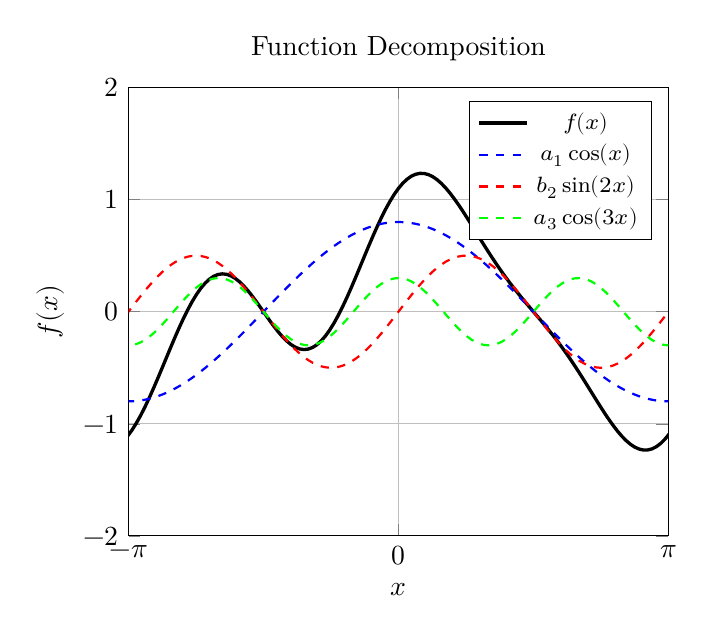
\begin{tikzpicture}
    \begin{axis}[
            xlabel={\(x\)},
            ylabel={\(f(x)\)},
            title={Function Decomposition},
            xmin=-3.14, xmax=3.14,
            ymin=-2, ymax=2,
            grid=major,
            legend pos=north east,
            samples=201,
            xtick={-3.14, 0, 3.14},
            xticklabels={\(-\pi\), \(0\), \(\pi\)},
            legend style={font=\footnotesize}
        ]

        % Example function to project
        \addplot[black, very thick] {0.8*cos(deg(x)) + 0.5*sin(deg(2*x)) + 0.3*cos(deg(3*x))};
        \addlegendentry{\(f(x)\)}

        % Individual basis functions scaled by their coefficients
        \addplot[blue, thick, dashed] {0.8*cos(deg(x))};
        \addlegendentry{\(a_1 \cos(x)\)}

        \addplot[red, thick, dashed] {0.5*sin(deg(2*x))};
        \addlegendentry{\(b_2 \sin(2x)\)}

        \addplot[green, thick, dashed] {0.3*cos(deg(3*x))};
        \addlegendentry{\(a_3 \cos(3x)\)}

    \end{axis}
\end{tikzpicture}
\end{document}
